{\color{red}
This chapter is intended to recapitulate the background of the thesis theme. In
Sec.~\ref{sec:2.1}, we recall the evolution of software systems with respect to
architecture and variability. In Sec.~\ref{sec:2.2} we outline the characteristics
of software performance, practical testing and measurement strategies as well as
some statistical background necessary to analyze, interpret and compare
performance assessment. In Sec.~\ref{sec:2.3} we present recent approaches for
feature model extraction from existing software systems and code artifacts. Finally, in
Sec.~\ref{sec:2.4} we recall and compare in detail different approaches to model
and predict performance behavior for configurable software systems.
}

\section{Variability Modeling}
The design and development of configurable software systems is conceptually
divided into \emph{problem space} and \emph{solution space} \citep{czarnecki_generative_2000}. The problem space
comprises the abstract design of features that are contained in the software system as well as
constraints defined among features, such as dependencies or mutual-exclusion.
The solution space describes the technical realization of features and the
functionality described by and associated with features, e.g., implementation
and build mechanisms. That is, features cross both spaces since they are mapped
to corresponding code artifacts.

A common way to express features and constraints in the problem space is to
define a \emph{variability model}, or \emph{feature model}, which subsumes all
valid configurations
\citep{kang_feature-oriented_1990,apel_feature-oriented_2013}. There are different and equivalent syntactical approaches to define feature models, for instance, a propositional formula $F$ over the set of
features of the configurable software systems \citep{batory_feature_2005}. In
this case a configuration is valid with respect to the feature model if and only if $F$ holds for all
selected features being true and all unselected features being false respectively. 
However, a more practical and more commonly used way to express feature models
are graphical tree-like \emph{feature diagrams}
\citep{apel_feature-oriented_2013}. In a feature diagram, features are ordered
hierarchically, starting with a root feature and subsequent child features. By
definition, the selection of a child feature requires the parent feature to be
selected as well. Child features can either be labeled as \emph{optional}
features  or \emph{mandatory} features; the latter ones need to be selected in
every configuration.
Moreover, feature diagrams
provide a syntax for two different types of feature groups, \emph{or-groups} and
\emph{alternative-groups}. For an or-group, at least one of the group's features
needs to be selected for a valid configuration, whereas for an alternative group
exactly one out of the group's mutually exclusive features must be selected. In
addition to the feature hierarchy, constraints, which cannot be expressed by
the tree-like structure, are referred to as \emph{cross-tree constraints}.
Cross-tree constraints, depending on the notation, are depicted by arrows
between two features or simply added to the feature diagram as a propositional
formula. For such two features $f_1$ and $f_2$, a cross-tree constraint means
that for feature $f_1$ to be selected, either the selection of $f_2$ is
required/implied or excluded.

An introductory example for the syntax and semantics of feature diagrams is
provided in Fig.~\ref{fig:introduction_fm}. In this example an imaginary
vehicle propulsion can be configured with eight valid configurations. The
vehicle requires an engine, and therefore feature \textsf{Engine} is mandatory.
At least one out of the three features \textsf{Hybrid}, \textsf{Piston} and \textsf{Electric} needs to be selected. For a piston engine, we can select either the feature \textsf{Diesel}
or \textsf{Petrol}. A petrol engine requires additional ignition sparks in
contrast to a Diesel engine. For an electric engine we require a
battery, hence, the feature \textsf{Battery} is mandatory.
In addition, the feature model specifies two cross-tree constraints: First, the
feature \textsf{Tank} is optional, yet once a piston engine is selected, we
require  a tank. Second, if we want to use the \textsf{Hybrid} functionality
(e.g., use both electric and piston engine simultaneously), we require to have both a piston
and an electric engine.

\begin{figure}[htbp]
  \centering
  
  	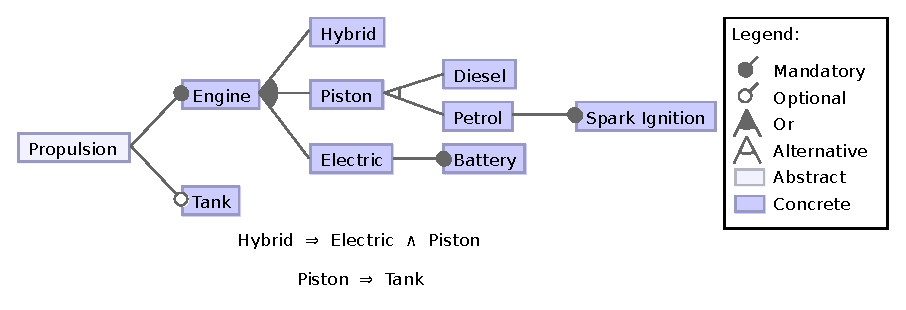
\includegraphics[width=0.75\textwidth]{images/introduction_fm.eps}
  \caption{Feature diagram for a feature model with eight valid configurations;
  two cross-tree constraints are specified as propositional formulas over
  features}
  \label{fig:introduction_fm}
\end{figure}

\section{Evolving Software} \label{sec:2.1}
\subsection{Software Evolution}
The first notion of the software development process is usually
developer-centered and merely focuses on software being designed, implemented,
tested, and eventually being released and deployed.
{\color{blue}Maintainability is a generally recognized software quality
property to look after, and maintenance is, of course, essential to every successful software system}. Nonetheless, less
attention is given to the ability to adapt a software system to changing
requirements (evolvability) rather than maintaining it to keep functionality
working \citep{parnas_software_1994}. Software evolution and evolvability, like
software itself are manifold. Software evolves in many ways ranging from maintenance (refactoring,
bug-fixes and patches) to adapting to changed requirements (adding, removing,
reorganizing functionality and variability).
Modern software systems not only often ship with a variety of configuration
options to select from, they also employ routines to be build and sometimes even
make use of or are part of platforms, such as apps or plugins. That is,
software evolution affects all aforementioned aspects, maintainability as
well as evolvability can degrade as software evolves.

\subsection{Software Erosion}
The negative symptoms of software evolution which are referred to as
``architectural erosion'' \citep{breivold_systematic_2012} have
been addressed by many researchers.
Most of existing research so far though focuses on evolution regarding software architecture
\citep{breivold_systematic_2012}. The main driving factors leading to symptoms of decay
identified by \cite{perry_software_1991} are architectural erosion and
architectural drift. While architectural drift subsumes developers'
insensitivity when not following a systems architecture or respective guidelines while making changes, architectural erosion subsumes ignoring and violating the existing software
architecture. \cite{parnas_software_1994} argues that as software evolves, software is maintained
and evolved by developers who are not necessarily familiar with the initial
architectural design. Therefore, knowledge about the architecture can become
unavailable. Although the unfavorable effects of software evolution do not necessary break a
system necessarily and imminently, the software becomes ``brittle'' \citep{perry_software_1991}
as maintainability as well as evolvability degrade. Concrete  symptoms of software
erosion on the implementation level have been documented. 

\cite{zhang_variability_2013} have studied erosion symptoms for a large-scale
industrial software product line with compile-time variability using
preprocessor directives.
The authors identify variability-related directives and clusters of those that
tend to become more complex as the software evolves. The negative effects, or symptoms of software
erosion are described as, but not limited to \emph{code replication} and
interdependencies between code elements, such as \emph{scattering} and
\emph{tangling}. Code scattering describes the phenomenon of code belonging to
a certain feature being scattered across multiple units of implementation,
e.g., modules, whereas code tangling means that code from different and
potentially unrelated features in entangled within a single module.

\cite{passos_feature_2015} have studied the extent of usage of scattering for device-drivers
in the Linux kernel. Despite scattering being quite prevalent, their
findings suggest that the kernel architecture is robust enough to have evolved
successfully. Nonetheless, platform drivers in the Linux kernel seem more
likely to be scattered than non-platform driver. They conclude that this is a
trade-off between maintainability and performance: a more generalized and
abstract implementation for platform-drivers in this case could possibly avoid
scattering, yet refactorings in this manner did not seem to be necessary or
worth the effort yet.

\subsection{Variability Evolution}
Apart from architecture evolution, the variability offered by software systems
evolves as well. For configurable software systems,
evolution steps will not only affect artifacts in the solution space, yet also
be visible in changes in the respective variability models in the problem space.
Although the variability aspect of software evolution has not gathered as
much attention as architecture in the past, more and more
research has emerged recently to address and understand variability evolution.

\cite{peng_analyzing_2011} proposed a classification of variability evolution patterns that
conceives evolution as adaption to changing (non-)functional requirements and
contexts. For a context in that sense, two categories exist. A driving context
determines, whether a variability model and respective variants can meet
functional requirements in the first place. A supporting context by definition
determines how non-functional properties are strengthened or weakened. 
Any changed requirement is likely to change the contexts for a software systems
variability model and, therefore, will make adaptations of the variability
model necessary. Within their classification method, \cite{peng_analyzing_2011} identify major
causes for variability evolution, comprising a) new driving contexts emerging, b) weakened supporting contexts (for instance, due to new
non-functional requirements), and c) unfavorable trade-offs for non-functional
properties. 

To understand single evolutionary steps, several catalogs of variability
evolution patterns have been proposed. \cite{peng_analyzing_2011} present three patterns,
where either a new feature is added, a mandatory feature becomes optional, or a
mandatory/optional feature is split into alternative features. \cite{seidl_co-evolution_2012} suggest a catalog of
patterns for co-evolution of variability models and feature mappings that additionally introduces code clones, splitting a feature
into more fine-grained sub-features and feature removal as evolution patterns.
In addition, \cite{passos_towards_2012} have studied variability evolution in
the Linux kernel and present a catalog of patterns where features are removed from the
variability model, but remain a part of the implementation. Their
catalog, among others, includes feature merges, either implicit (optional feature merged
with its parent) or explicit.

The classification proposed by \cite{peng_analyzing_2011} is a general and formalized approach
that, as well as \cite{seidl_co-evolution_2012} and \cite{passos_towards_2012}, describes
elementary evolution patterns which can be composed to more complex patterns. Nonetheless, no
comprehensive catalog of variability evolution so far has been proposed.

\section{Feature Model Synthesis}  \label{sec:2.3}
A variability model as an abstraction of functionality of a software system is
required, or at least of great interest, in many contexts. 

\emph{First}, not
every configurable system provides an explicit
representation of its variability model. 
The reasons for inexplicit or absent configuration specification are manifold.
They can range from poor or inconsistent documentation
\citep{rabkin_static_2011} to overly complex configurability
\citep{xu_hey_2015}, or configuration constraints originated in different layers of a software
system, e.g.m build constraints  or compiler constraints \citep{nadi_where_2015}. 

\emph{Second}, variability models have emerged to be a useful means in domain
analysis prior to developing a software system. {\color{blue}As variability
models group and organize functionality, synthesizing a variability model has shown to be
applicable to extract features and constraints from functional requirements. 
In addition, by comparison of product specifications for an
existing market domain, variability models can provide detailed feature
summary.}

For this thesis, we focus on the first aspect of synthesizing variability
models as our work addresses the assessment of already existing configurable
software systems. Nonetheless, many techniques employed in the aforementioned
second aspect address similar problems, yet rely on natural language artifacts
rather than code artifacts \citep{alves_exploratory_2008,bakar_feature_2015}.
The following section recalls work on extracting configuration options and
constraints from source code as well as the organization of constraints into
feature hierarchy and groups. The further assessment of configurable systems
requires a well-defined and sound variability model.

\subsection{Feature Extraction} 
The first objective in recovering a variability model from a configurable
system is to determine the available configuration options to select
from. In addition, for further configuration, the type of each configuration
option (e.g., boolean, numeric or string) and the respective domain of valid values
needs to be specified.

\cite{rabkin_static_2011} proposed a static, yet heuristic approach to extract
configuration options along with respective types and domains. Their approach
exploits the usage of configuration APIs and works
in two stages. It commences with extracting all code sections where
configuration options are parsed. Next, configuration names can be
recovered as they are either already specified at compile-time or can be
reconstructed using string analysis yielding respective regular expressions.
Moreover, the authors employ a number of heuristics to infer the type of parsed
configurations as well as respective domains. First, the return type of the
parsing method is likely to indicate the type of the configuration option read.
Second, if a string is read initially, the library method it is passed to can
reveal valuable information about the actual type. For instance, a method
\emph{parseInteger} is likely to parse an integer value. Third, whenever a
parsed configuration option is compared against a constant, expression, or value
of an enum class, these might indicate valid values or at least corner cases of
the configuration option domain. The extraction method by
\cite{rabkin_static_2011} is precise, but limited, for instance, when an
option leaves the scope of the source code.
Nonetheless, for the systems studied, the authors recovered configuration
options that were not documented, only used for debugging or even not used at
all.

\subsection{Constraint Extraction}
The second step in recovering a variability model is the
extraction of configuration constraints. An approach proposed by \cite{zhou_extracting_2015}
focuses on the extraction of file presence conditions from build files using symbolic execution. A more comprehensive investigation of configuration
constraints and their origin is provided by \cite{nadi_mining_2014,nadi_where_2015}. They
propose an approach based on variability-aware parsing and infer constraints by
evaluating make files and  analyzing preprocessor directives. Inferred
constraints result from violations of two assumed rules, where a) every valid
configuration must not contain build-time errors and b) every valid
configuration should result in a lexically different program, thus. While the
first rule aims at inferring constraints that prevent build-time errors, the
second one is intended to detect features without any effect, at least as part
of some configurations. Their analysis one the one hand emerged to be accurate
in recovering constraints with 93~\% for constraints inferred by the first rule
and 77~\% for second one respectively. On the other hand, their approach
recovered only 28~\% of all constraints present in the software system.
Further qualitative investigation, including developer interviews, lead to
the conclusion that most of existing constraints stem from domain knowledge
\citep{nadi_where_2015}.

\subsection{Feature Hierarchy Recovery} 
Besides recovering configuration options and respective constraints, to reverse
engineer a feature model, one further step is required. The recovered knowledge
needs to be organized in a tree-like hierarchy with feature groups specified and
CTCs explicitly stated to derive a valid feature diagram 
\citep{kang_feature-oriented_1990}.
While several approaches to the recover feature model hierarchy have been proposed, we are primarily interested in finding a hierarchy for knowledge obtained from
source code. Other scenarios, as already stated in the opener of this section,
are based on product descriptions or sets of valid configurations. The remainder of
this subsection we will focus on organizing features and constraints extracted
from source code. For further reading, \cite{andersen_efficient_2012} present
algorithms for structuring feature diagrams for three different scenarios including the
ones previously mentioned.

Given an extracted set of features along with corresponding descriptions and
recovered constraints among the features, \cite{she_reverse_2011} propose a
semi-automated and interactive approach to synthesize a feature hierarchy.
Their approach comprises three tasks. First, an overall feature hierarchy based
on feature implications is specified. Second, potential feature groups are
detected and manually selected. Finally, the feature diagram is extended with
remaining CTCs. A detailed decription of the algorithm is presented below:

\begin{enumerate}
  \item The algorithm commences with finding a single parent for each
  feature and, thus, specifying a tree-like feature hierarchy. Based on the
  given constraints a directed acyclic graph (DAG) representing implication
  relationships among features, a so-called implication graph, is constructed.
  Every vertex in the implication graph represents a feature  and edges are
  inserted for each pair of features $(u, v)$, where  $u \implies v$ holds with respect to the given
  constraints.
   
  In addition to the implication graph, the algorithm for each feature computes
  two rankings of features that are likely to be the respective parent feature.
  The two rankings both employ the feature descriptions. Feature descriptions
  are compared for similarity using a similarity metric. For two features $p$
  and $s$ the similarity is defined as the weighted sum of the inverse document
  frequencies $idf(w)$ for the words that both descriptions of features $p$
  and $s$ share.
  The $idf$-ranking for a word $w$ is the logarithm of the number of features
  divided by the number of features whose description contains $w$. Each $idf$
  value is weighted with the frequency of $w$ in the description of
  feature $p$.
  
  The first ranking, called Ranked-Implied-Features (RIF), for each feature $f$
  ranks all features by their similarity to $f$ in an descending order, but
  prioritizes those features that are implied according to the previously
  computed implication graph. The second ranking, called Ranked-All-Features
  (RAF) is similar to RIF, yet less strict since implied features are not
  prioritized. Given these rankings, a user for each feature selects a suitable
  parent feature from the RIF or RAF ranking. The idea behind providing two
  separate rankings, according to \cite{she_reverse_2011} is that the given
  extracted constraints can be incomplete and, thus, not all relevant
  implications are contained in the implication graph.

  \item After the feature hierarchy is specified, another auxiliary graph, a
  mutex graph, similar to the implication graph, is constructed. The mutex
  graph is an undirected graph with features as vertices and edges between two
  features $u$ and $v$, if $u \implies \neg{v}$ and $v \implies \neg{u}$ hold
  with respect to the given constraints. 
  That is, all adjacent features are mutually exclusive. Based on
  this mutex graph all maximal cliques (subsets of vertices that all are
  connected with each other) among the vertices with the same parent are
  computed. All features within such a clique are mutually exclusive and share
  the same parent and represent mutex- or alternative-groups. \cite{she_reverse_2011} introduce an
  additional constraint to extract xor-groups that require one of the groups’
  features to be selected if the parent is selected. This distinction is in
  line with the initial description of feature diagrams by \cite{kang_feature-oriented_1990},
  but not all descriptions of feature diagrams follow this distinction between
  mutex- and xor-groups and just use the term alternative-group discussed in 
  Sec. \ref{}. %2.1
  
  \item CTCs for the feature diagram are extracted from
  the given configuration constraints. Since CTCs are constraints that could
  not be represented by the feature hierarchy (implication) or
  alternative-groups (exclusion) the derivation of CTCs follows this idea. The
  set of cross-tree implications is derived by removing all edges that are part
  of the feature hierarchy from the initially constructed implication graph.
  The set of cross-tree exclusions is derived in the same manner from the mutex
  graph by removing all edges among vertices of all mutex-groups. To make the
  feature model sound, the given configuration constraints, reduced to those
  clauses that are not already entailed by the diagram, can be added as an
  additional CTC formula to the feature diagram \citep{she_reverse_2011}.
\end{enumerate}

The approach by \cite{she_reverse_2011} provides a practical algorithm to synthesize a
feature diagram, yet has some aspects we might need to consider. First, the
approach is not able to detect or-groups as defined in Sec. \ref{}. Second, the
approach does introduce a root feature. Finally, the approach does not
distinguish between mandatory and optional features. Implicitly, all features
that do not have a parent feature are optional and all features that have a
parent feature are by default mandatory. \cite{she_reverse_2011} evaluated the
algorithm with both complete and incomplete variability knowledge (feature
names, descriptions and constraints). While the algorithm has shown to be
practical, detecting features whose parent was the root-feature was difficult
since, due to the transitive property of implication, it is implied by each
feature of the feature model.

\section{Assessing Performance} \label{sec:assessing_performance}
While the last three sections covered software evolution and variability
modeling, we now step forward to the topic of software performance. This
section will outline the term performance with respect to software systems as
well as to possible measurements. We provide a brief look at the general performance
testing setup and the required prerequisites, including suitable benchmarks.
Finally, we provide the statistical background to summarize, interpret and
compare performance measurements accurately.

\subsection{What is Performance?}
The performance of software systems is, like software quality, primarily a
matter of perspective. While an end user might consider practical aspects to be
more important, from a developer’s perspective, performance relates to and is
best described by non-functional properties \citep{molyneaux_art_2014}.
{\color{blue}While functional properties subsume what exactly a software system does, non-functional
properties describe how (good or bad) a software system is at providing the
functionality offered}. The notion of good and bad in this sense corresponds to
non-functional requirements (NFR), that is, software with good performance
behavior satisfies NFRs. The categories of NFRs that shape performance behavior
are manifold. According to \cite{molyneaux_art_2014}, the categories or
\emph{key performance indicators} (KPIs) include 

\begin{itemize}
  \item availability
  \item response time,
  \item throughput,
  \item resource utilization, and in a broader scope also 
  \item capacity.
\end{itemize}

Time-related KPIs are availability and response time, whereby
availability describes the time or time ratio that the software is available to
the end user, and response time subsumes the time it takes to finish a request
or operation. Throughput as a category subsumes the program behavior with
respect to program load, such as hits per second for a web application or
amount of data processed per second. Resource utilization describes the extent
to which a software system uses the physical resources (CPU time, memory, and
disk or cache space) of the host machine. Finally, from a web-centered
perspective, capacity describes measurements with respect to servers and
networks, such as network utilization  (traffic, transmission rate) and server
utilization, such as resource limitations per application on a host server
\citep{molyneaux_art_2014}.

Consequently, the assessment of performance requires a context or testing
target that corresponds to the assessed system under test (SUT). For instance,
for a simple command-line compression tool, suitable KPIs are response time and
throughput, whereas performance for an online shop web application is better
outlined by availability and capacity.

\subsection{Performance Testing}
The first step in performance testing, prior to defining relevant KPIs and
metrics, is to specify a system operation or use case \citep{woodside_future_2007} to
assess performance for. A typical use case includes a well defined task or
workload to process, expected behavior, outcome, and performance
requirements as previously discussed. For the SUT, however, we require a
version that does compile or, in case it is interpreted, is syntactically
correct \citep{molyneaux_art_2014}. With regard to performance assessments as part of
the development process, a code freeze should be obtained since measurement
results are likely to become meaningless for later versions. In addition to
that,  the machine or setup used for performance measurement should ideally be
as close to the production environment as possible, but at least be documented
to compare different runs \citep{molyneaux_art_2014}.

Finally, one or more benchmarks need to be selected to simulate  the program
load for the respective use case. A benchmark, all in all, needs to be
representative, i.e., should relate to the the use case or requirement one
 wants to validate. While benchmarks for file compression usually include
multiple different types of media data (text, sound, pictures) like the
{\color{blue}Canterbury corpus\footnote{bener}}, web applications can be exposed
to dealing with a number of simulated users at the same time \citep{molyneaux_art_2014}. Benchmarks have often been
standardized within research and engineering communities to provide comparable
performance measurements. A popular example is the Software Performance Evaluation
Corporation (SPEC), a consortium providing a variety of benchmarks like the
CPU2000\footnote{The benchmark description
can be found at \url{https://www.spec.org/cpu2000/}.} processor benchmark
consisting of programs with both floating point and integer operations.
Moreover, benchmarks in a sense of repeatable program load can be obtained from
load generation software like ApacheBench\footnote{Manual page of the Apache
tool \texttt{ab}, \url{http://httpd.apache.org/docs/2.4/en/programs/ab.html}.}
for the Apache web server or simply by measuring performance for test cases
\citep{heger_automated_2013,nguyen_industrial_2014}.

Performance testing heavily relies on tool support, especially for repeating
test cases and recording measurements. Since the
tool solutions for performance testing vary from domain, scale and purpose, we
will only outline the general tool architecture. \cite{molyneaux_art_2014} describes
four primary components for a performance testing setup: a scripting module, a
test management module, a load injector, and an analysis module. A scripting module handles the generation or
repetition of use cases which, for instance, can be recorded prior to the test
for web applications. A test management module creates and executes a test
session, whose program load is generated by one or more load injectors. A load
injector can provide a benchmark by generating items to process, or can simulate
a number of clients for a server-side application. An analysis module, finally,
collects and summarizes data related to the performance testing target. More on
summarizing and comparing recorded results in the next section.

\section{Statistical Considerations}
In this section we now discuss the appropriate statistical means to summarize,
compare and interpret measurement results. For the remainder of this section we
will refer to the following two use cases. First, to obtain robust results, the
assessment of a single variant needs to be repeated multiple times.
Consequently, to report a single result per metric, the measurements for a
single variant need to be summarized. Second, the assessment of performance for
a variant may comprise several use cases or system operations, for instance file
compression and decompression for a compression software. Therefore, performance measures
aggregated from different benchmarks need to be summarized accurately. 

\subsection{Measures of Central Tendency}
For each test run of a software system or variant, we obtain a single-valued
measurement per performance metric. Since we repeat each test run $n$ times
per variant, we obtain a data record $X$ with $n$ measurements $X = X_1, X_2,
\ldots, X_{n-1}, X_n$. While the arithmetic mean is commonly considered the
right means to summarize data records and report a representative average
value, we need to be more cautious with how to summarize data records
\citep{fleming_how_1986,smith_characterizing_1988}. From a statistical
perspective, the intention of summarizing a data record is to find a measure of
central tendency what is representative for the data record.
While the arithmetic mean is an appropriate method for many cases, there exist
other means to summarize data records. Moreover, there exist a number of
criteria for when to use which means to summarize a data record. 

The first question when summarizing a data
record is to ask what the data actually describe and what we to express with our
summary. For a data record $X$, we can define a
relationship we would like to keep while replacing each single $X_i$ with an
average value $\bar{x}$. Based on this relationship, we can derive the
appropriate method to summarize our record. For instance, our data record $X$
describes the time elapsed for a test case and we want the keep the following
relation, saying that the sum of all measurements $\sum_{i = 1}^{n}$ is defines
the total time elapsed $T$ as

$$
T = \sum_{i = 1}^{n} X_i = \sum_{i = 1}^{n} \bar{x}.
$$

Based on the term above, we can derive the definition of the method
appropriate to summarize our data record with respect to the conserved relation
what is the \emph{arithmetic mean}, defined as

\begin{equation} \label{eq:arithmetic_mean}
\begin{split}
\bar{x} = \frac{1}{n} \sum_{i = 1}^{n} X_i.
\end{split}
\end{equation}

Consider another example, similar to the one above, where the test
case is a load test with a predefined number of users and the measurements $X =
X_1, X_2, \ldots, X_{n-1}, X_n$ are
measured as hits per second. Again, we have different measurements we want to
summarize with respect to a relation to conserve. Each user drops the same
number of requests $T$, whereby the hit rate $X_i$ and the respective elapsed
time $t_i = \frac{T}{X_i }$ vary. We now conserve the relationship that the
total number of requests for the data record is the sum of all hit rates $X_i$
times the time elapsed $t_i$. Therefore, we want to substitute each hit rate
$X_i$ with an average value $\hat{x}$ so that the aforementioned rule holds

$$
n\cdot T - \sum_{n}^{i=1} X_it_i = 0 \Leftrightarrow n\cdot T - \hat{v}
\sum_{n}^{i=1} t_i = 0 \Leftrightarrow n = \hat{x} \sum_{n}^{i=1} \frac{1}{X_i}
$$

Similar to Eq. \ref{eq:arithmetic_mean} we can derive the definition for the summarization
method to use from the equation above what is the \emph{harmonic mean}, defined as

\begin{equation} \label{eq:harmonic_mean}
\begin{split}
\hat{x} = n \cdot \bigg(\sum_{i=1}^{n} \frac{1}{X_i}\bigg)^{-1} =
\frac{n}{\frac{1}{X_1} + \frac{1}{X_2} + \ldots +
\frac{1}{X_{n-1}} + \frac{1}{X_n}}.
\end{split}
\end{equation}

We see that the summarization methods presented in Eq. \ref{eq:arithmetic_mean}
and \ref{eq:harmonic_mean} are useful for different types of data records and they should
be used accordingly. The arithmetic mean is suitable for records, where the total sum of single
measurements has a meaning, whereas the harmonic mean is suitable for measured
rates or frequencies \citep{smith_characterizing_1988}.

While the aforementioned measures of central tendency should be appropriate for
most cases, they are not always the best choice though. The arithmetic
and harmonic mean are heavily influenced by extreme observations
\citep{shanmugam_statistics_2015}. 
For instance, for the data record $X = 1, 2, 3, 30$ three of four values are smaller than the
arithmetic mean $\bar{x} = 9$. One option is to explicitly exclude outlier
values from the data record. The so-called \emph{trimmed mean} is
obtained by truncating a upper and/or lower percentage $t$ of the data record
and, consequently, computing the (arithmetic or harmonic) mean for the remaining
data record \citep{shanmugam_statistics_2015}. 

While this method is suitable to omit the effects of outliers, one still needs to specify
which upper and/or lower percentage $t$ needs to be truncated. Moreover, the use
a (trimmed) mean requires the data records' frequencies to be distributed
symmetrically around its mean.
A probability distribution is skewed (and therefore asymmetric) if, graphically speaking, its histogram is not
symmetric around its measure of central tendency. A simple method to measure the
skewness of a probability distribution is \emph{Bowley's measure}
\citep{shanmugam_statistics_2015}, defined as

\begin{equation} \label{eq:bowley}
\begin{split}
B_S = \frac{(Q_3 - M) - (M - Q_1)}{Q_3 - Q_1} = \frac{(Q_3 + Q_1 - 2M)}{Q_3
- Q_1},
\end{split}
\end{equation}

where $Q_1$ and $Q_3$ denote the first and third quartile, and $M$ denotes the
median of the probability distribution. The quartiles $Q_i$ with $i \in \left\{
1,2,3 \right\}$ are defined as the values of a data record $X$, so that
$\frac{i}{4}$ of the values of $X$ are smaller than $Q_i$. The \emph{median} is
defined as $Q_2$, i.e., a value $M \in X$ so that half of the values in $X$ are smaller than $M$.

The median itself is a more robust measure of central tendency than the
aforementioned ones since it is less influenced by outliers and can be used for
both skewed and symmetric data records \citep{shanmugam_statistics_2015}. For a
given ascendingly ordered data record $X = X_1, X_2, \ldots, X_{n-1}, X_n$, we
can compute the median as follows:

\begin{equation} \label{eq:median}
\mathrm{Median}(X) = \begin{cases}
     X_{\frac{n+1}{2}} & \text{if $n$ is odd} \\
     \frac{1}{2}\big(X_{\frac{n}{2}} + X_{\frac{n}{2}+1}\big) & \text{if $n$ is
     even}
   \end{cases}~\text{with $X_i \leq X_j$ and $i < j \leq n$ }
\end{equation}

\subsection{Measures of Dispersion}

Last, we take a look at different measures of spread or dispersion. Most
commonly used are the \emph{variance} $\sigma^2$ and the \emph{standard
deviation} $\sigma = \sqrt{\sigma^2}$ defined along the mean $\mu$ of a
probability distribution as

\begin{equation} \label{eq:variance}
\begin{split}
\sigma^2 = \frac{\sum_{i=1}^{n}(X_i - \mu)^2}{n}
\end{split}
\end{equation}

Similar to the (arithmetic or harmonic) mean, the variance and the standard
deviation are heavily influenced by extreme observations
\citep{shanmugam_statistics_2015} are not the best choice in all cases. Instead,
two more robust measures are the \emph{median absolute deviation} (MAD) and the \emph{inter-quartile range} (IQR). The MAD is defined as the median of the absolute deviations from the probability distributions'
median \citep{molyneaux_art_2014}, or, defined as follows:

\begin{equation} \label{eq:mad}
\begin{split}
\mathrm{MAD}(X) = \mathrm{Median}\big(|X - \mathrm{Median}(X)|\big)
\end{split}
\end{equation}
 
The IQR, however, defines the range between the first and the third quartile
$Q_1$ and $Q_3$ \citep{shanmugam_statistics_2015}. This range is larger for a
widespread data record and smaller for a data range with a narrow spread, but is not influenced by extreme
observations as those outliers do not lie within the range $\left[ Q_1,Q_3
\right] $. The IQR is defined as follows

\begin{equation} \label{eq:iqr}
\begin{split}
\mathrm{IQR}(X) = Q_3 - Q_1.
\end{split}
\end{equation}

\subsection{When to use which measure?}
In this section we discussed the arithmetic and harmonic mean as well as the
median as a measure of central tendency, the symmetric property that is
required to use the arithmetic or harmonic mean, and different measures of
spread for a given data record. At the beginning we asked for means to
summarize data records a) for an experiment repeated multiple times, and b)
obtained from different benchmarks. While for case b) the answer is to use the
arithmetic or harmonic mean (depending on the quality of the measurements), for
a) the answer is a little more elaborate.

The arithmetic (or harmonic) mean can be used whenever the quality of the
measurement is appropriate and the data record is symmetric. According to
\cite{shanmugam_statistics_2015}, the arithmetic mean is preferable ``when the numbers combine
additively to produce a resultant value'', such as time periods or memory sizes, whereas
the harmonic mean is preferable ``when reciprocals of several nonzero numbers
combine additively to produce a resultant value'', such as rates or frequencies
\citep{smith_characterizing_1988}.
The median is a less precise estimator than the both means, yet more robust
with regard to extreme observations. In addition, the MAD or IQR provide a more
robust means of spread than the standard deviation.

\section{Performance Prediction Models}
\label{sec:performance-prediction-models} 
In the last section we referred to performance, or in detail, the KPIs, as
possible testing targets we validate against non-functional requirements.
However, in a broader sense, software performance has become an aspect of
software engineering referred to as \emph{software performance engineering}
(SPE) \citep{woodside_future_2007}.
A lot of effort has been spent to study and describe performance behavior as well
as to improve performance quality. Besides the analysis of concerns or
requirements with respect to performance, SPE comprises performance testing as
well as performance prediction \citep{woodside_future_2007}. Performance
prediction aims at modeling and estimating performance behavior for different
use cases or configurations. The first approaches to performance prediction models model the underlying software system component or operation from which
performance estimations are then deduced. These so-called \emph{model-based prediction models} enable a
performance estimation early in the development process since no actual
performance measurement is required \citep{woodside_future_2007}. In opposition
to model-based approaches, measurement-based approaches have emerged. These \emph{measurement-based prediction models} are based on a sample of performance
measures which are used to learn a software systems’ performance behavior
\citep{woodside_future_2007}. More recently, measurement-based prediction models that emphasize variability have been
proposed, of which we will discuss three approaches in the remainder of
this section.

\paragraph{Learning Performance} In essence, learning and predicting performance
behavior for a configurable system means nothing different than finding an approximation $h$ for a function
$f: C \rightarrow \mathbb{R}$ where $C$ is the set of configurations and $f(c)
\in \mathbb{R}$ with $c \in C$ is the corresponding performance measurement. The
accuracy of the approximation $\hat{f}$ describes how the estimated performance
$\hat{f}(c)$ deviates from the actually measured performance $f(c)$. 
Different approaches to construct such an approximation, referred to as a
\emph{performance prediction model}, emerged recently. All approaches utilize
two samples of configurations and corresponding performance
measurements to build and validate the model. A training sample is used to
learn the approximation from, whereas a testing sample is used to assess the
prediction error rate of the previously learned approximation.
%While the
%approaches mentioned below differ in the expression of a performance prediction
%model, all require ``meaningful'' training samples and stress the importance of
%sampling strategies.

A straightforward
methodology to learn performance behavior was proposed by \cite{guo_variability-aware_2013}. The
authors utilize classification-and-regression-trees (CART), akin to decision
trees, to derive a top-down classification hierarchy for a given sample. The
approach supports progressive (and random) sampling, i.e., the performance
model is constructed several times while the size of the training sample is
successively increased. The model construction commences with a recursive
segmentation to find an an accurate CART for a local subset of the training
sample. Subsequently, the local trees are merged to constitute a CART for the
whole training sample. It is worth mentioning that the estimation using CART is
not limited to binary configuration options, but supports numeric features as
well. Moreover, the approach by \cite{guo_variability-aware_2013} does not produce any further
computation overhead besides the measurement effort and the construction of a
CART.

A different approach to modeling performance behavior was
proposed by \cite{zhang_performance_2015}. The authors propose an approach to construct
performance prediction models based on a Fourier description of the
performance-describing function $f$. The principal idea is to approximate a
Fourier series approximating the function performance-describing $f$, and
learning all coefficients of the series terms.
The number of terms is exponential in the number of configuration options. The main
characteristic of this approach is that, prior to learning a performance
prediction model, a desired level of prediction accuracy can be specified. That
is, the approach automatically chooses the sample size required to learn the
prediction model accordingly.

A third approach to model and predict performance behavior,
\emph{SPLConqueror}, was proposed by \cite{siegmund_predicting_2012}. The
authors describe performance behavior  for a configuration as the accumulated influence of
features the configuration is composed from, and respective feature
interactions. To estimate the influence of single features and feature
interactions, the authors propose a number of sampling strategies. Single
features are assessed by comparing the performance of two different
configurations per feature: For a feature $f$, two valid configurations are
compared, whereby both configurations have the minimal number of features
selected that are not excluded by the selection of $f$. While for one
configuration $f$ is selected, it is deselected for the other one. The
difference between the performance measures for both configurations is the estimate
$\Delta_{min(f)}$ for the performance influence of feature $f$. Feature
interactions that are performance-relevant are detected automatically in a similar manner. The
main idea is, that a feature $f$ is more likely to interact with other features,
the more features are selected along with $f$. Therefore, if $f$ interacts, the
influence of feature $f$,  $\Delta_{min(f)}$ differs from the influence of $f$,
when estimated using configurations where the maximal number of features selectable
together with $f$ are used. Based on the set of interacting features, three
heuristics are employed to detect feature interactions. Simple feature
interactions are detected using pair-wise sampling
\citep{siegmund_predicting_2012,apel_feature-oriented_2013}, whereas
higher-order feature interactions are often composed from simpler ones, or centered
around a small subset of hot-spot features \citep{siegmund_predicting_2012}.
Finally, for an arbitrary configuration the performance can be predicted by the sum of influence
estimations per feature and feature interaction.

The idea of predicting performance by estimating the influence of feature
and feature interactions was further developed by \cite{siegmund_performance-influence_2015} by
proposing performance influence models for both binary and numeric
configuration options. A performance influence, similar to \emph{SPLConqueror},
predicts performance by computing the sum of previously learned influence
estimates. The novelty of this approach lies in the way the terms describing
the influence of feature and feature interactions are learned and not
derived from a sampling strategy.
Instead of a single constant performance influence estimate, each term can contain of a
number of functions, such as linear, quadratic or logarithm functions, or
compositions thereof. This does not only allow to incorporate domain knowledge
by preselecting functions. Moreover, by introducing combinations of non-linear
functions and learning the coefficients using linear regressions enables
learning a non-linear function. The algorithm commences with the selection of
terms and successively extends and reduces the term selection to increase 
the prediction accuracy. The outcome, similar to
\cite{siegmund_predicting_2012}, is a linear function whose terms represent the estimated influence of features and
feature interactions on performance.

All aforementioned approaches rely on performance measurements and, to
some extent, also on a  sampling strategy. While the approaches by
\cite{siegmund_predicting_2012,siegmund_performance-influence_2015} essentially describe sampling strategies,
the approach proposed by \cite{zhang_performance_2015} is able to work with random samples, and the
approach of \cite{guo_variability-aware_2013} does extend its training sample automatically. As
performance measurements entails an expensive and time-consuming process,
\cite{sarkar_cost-efficient_2015} have investigated different sampling
strategies in this domain.
The authors compare progressive sampling, where sample sizes are increased
successively until the learned prediction model performs accurately enough, and projective
sampling, where the optimal sample size is estimated based on the expected
learning curve, with respect to cost and prediction accuracy. They advocate the
use of projective sampling over progressive sampling. In addition, the authors
propose and evaluate an own sampling heuristic to select an initial sample for
progressive sampling. This sampling heuristic is based on feature frequencies
and outperforms t-wise sampling, such as pair-wise sampling
\citep{sarkar_cost-efficient_2015}.